\documentclass[a4paper]{siamart220329}

\usepackage{damacros}

% Theorem environment for questions: Small-caps header, italize body.
\theoremstyle{plain}
% \theoremheaderfont{\normalfont\sc}
\theoremheaderfont{\normalfont\bf}
\theorembodyfont{\normalfont}
\theoremseparator{.}
\theoremsymbol{}
\newtheorem{question}{Question}
\crefname{question}{Question}{Questions}
\Crefname{question}{Question}{Questions}

\usepackage{listings}
\definecolor{LightGrey}{rgb}{0.9629411,0.9629411,0.9629411}
\definecolor{LighterGrey}{gray}{0.99}
\definecolor{Mauve}{rgb}{0.58,0,0.82}
\definecolor{Emerald}{rgb}{0.31, 0.78, 0.47}
\definecolor{RoyalBlue}{rgb}{0.25, 0.41, 0.88}
\definecolor{myGreen}{cmyk}{0.82,0.11,1,0.25}
\lstset{
    language=Matlab,
    keywordstyle=\color{RoyalBlue},
    basicstyle=\ttfamily,
    morekeywords={define,ifndef,endif},
    commentstyle=\color{myGreen}\small\ttfamily,
    %directivestyle=\color{Mauve}\scriptsize\ttfamily,
    showspaces=false,            
    showstringspaces=false,
    stringstyle=\color{Mauve}\ttfamily,
    numbers=left,
    numberstyle=\scriptsize,
    stepnumber=1,
    numbersep=8pt,
    showstringspaces=false,
    breaklines=true,
    frameround=ftff,
    frame=lines,
    backgroundcolor=\color{LightGrey}
} 
\usepackage{xr}
\externaldocument[T1-]{../../Tutorial1/Questions/tutorial-01}

% Sets running headers as well as PDF title and authors
\headers{Tutorial 2}{D. Avitabile}

% Title. If the supplement option is on, then "Supplementary Material"
% is automatically inserted before the title.
\title{Nonlinear Dynamical Systems Part 3 \\ 
  Dynamics in pattern-forming systems \\
  Tutorial 2
} 

% Authors: full names plus addresses.
\author{%
  Daniele Avitabile%
  \thanks{%
    Vrije Universiteit Amsterdam,
    Department of Mathematics,
    Faculteit der Exacte Wetenschappen,
    De Boelelaan 1081a,
    1081 HV Amsterdam, The Netherlands.
  \protect\\
    Inria Sophia Antipolis M\'editerran\'ee Research Centre,
    MathNeuro Team,
    2004 route des Lucioles-Boîte Postale 93 06902,
    Sophia Antipolis, Cedex, France.
  \protect\\
    (\email{d.avitabile@vu.nl}, \url{www.danieleavitabile.com}).
  }
 % \and
%   Paul T. Frank \thanks{Department of Applied Mathematics, Fictional University, Boise, ID 
% (\email{ptfrank@fictional.edu}, \email{jesmith@fictional.edu}).}
% \and Jane E. Smith\footnotemark[3]
}

\begin{document}

\maketitle

\begin{abstract}
  Themes of of this tutorial:
  \begin{enumerate}
    \item Inferring bifurcation diagrams using brute-force simulation (and its perils)
    \item Numerical solution of boundary-value problems
    \item Performing numerical continuation 
    \item Numerical study of linear stability of steady states
  \end{enumerate}
\end{abstract}

\section{Introduction}
In this tutorial we will continue working with the following Allen--Cahn PDE, subject to
homogeneous Neumann (no-flux) boundary conditions
\begin{equation}\label{eq:AC}
  \begin{aligned}
    & \partial_t u = \nu \partial_{xx}u + \lambda u + \alpha u^2 + \beta u^3 - \gamma
    u^5, & & (x,t) \in (-5,5) \times \RSet_{>0}, \\
	& \partial_x u(-5,t) = \partial_x u(5,t) = 0, && t \in \RSet_{\geq 0}, \\
	& u(x,0) = \varphi(x), && x \in [-5,5].
  \end{aligned}
\end{equation}

In Tutorial 1 we have derived, implemented, and time stepped a set of $n$ coupled ODEs
approximating \cref{eq:AC}, %in the form
\begin{equation}
  \dot U = F(U,p), \qquad U(0) = \{ \varphi(x_i) \}_{i=1}^n
\end{equation}
where $U(t) \in \RSet^n$, contains an approximation to $u(x,t)$ at $n$ grid points 
$\{ x_i \}_{i=1}^n$ in $[-5,5]$, $p = (\nu,\lambda,\alpha,\beta,\gamma) \in \RSet^5$ is a
vector containing all control parameters, and $F \colon \RSet^n \times \RSet^5 \to
\RSet^n$. 

Henceforth we will fix $\nu = \beta = \gamma =1$, $\alpha=0$, and use $\lambda$ as
principal continuation parameter. Owing to this convention we may write, with a
slight abuse of notation, $F(u,\lambda)$ and $F(u,p)$ interchangeably.

\begin{question}[Time simulations and bifurcation diagrams]
\begin{figure}[t!]
  \centering
  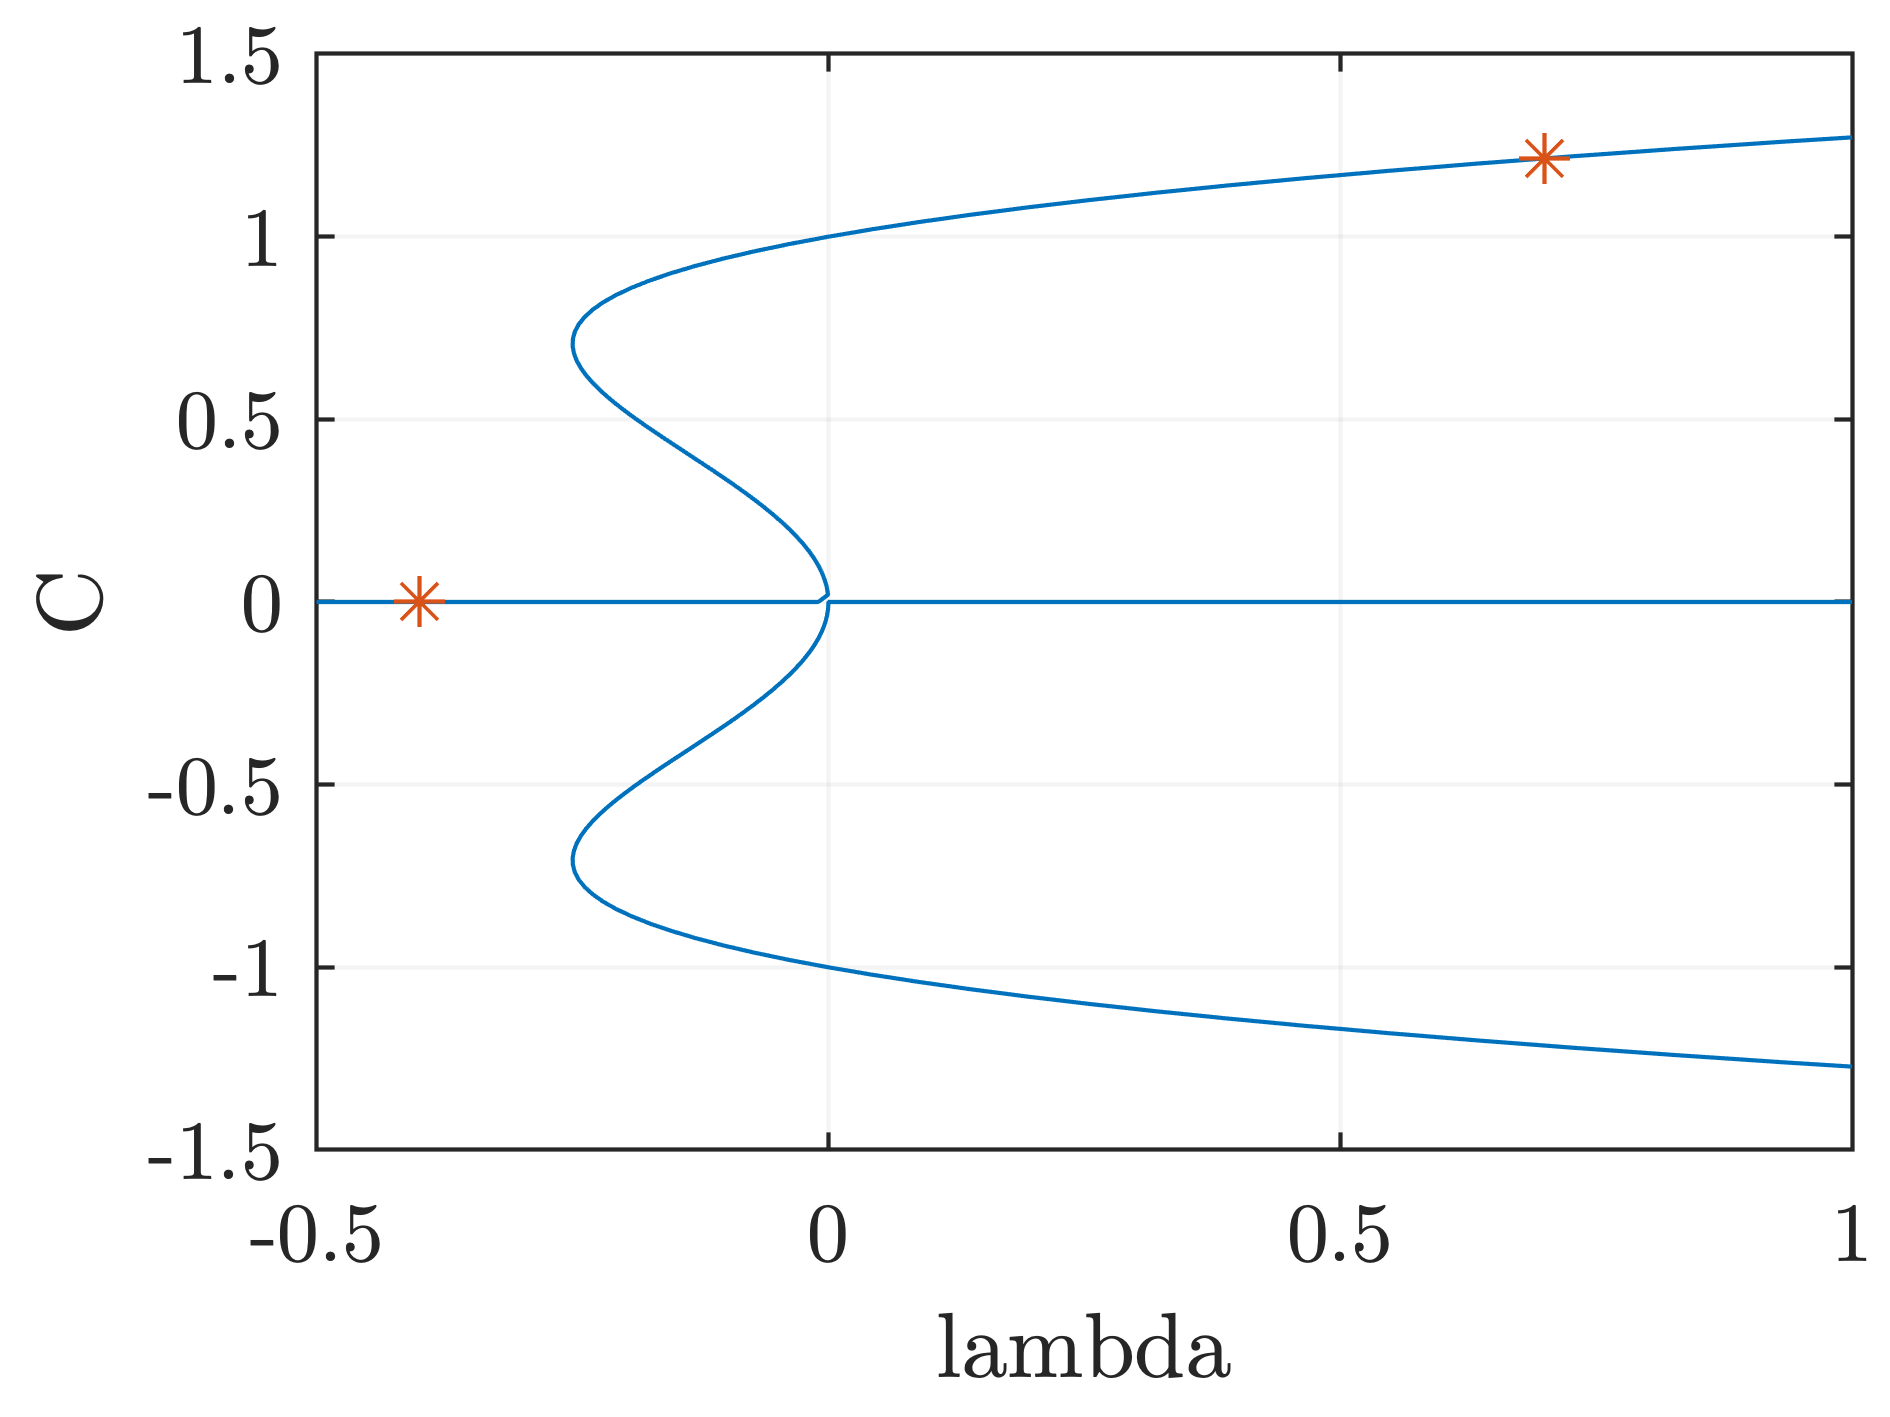
\includegraphics{bd_hom}
  \caption{Equilibria of homogeneous steady states in the parameter
  $\lambda$ and solution measure $S_1 = C$ for \cref{eq:AC} with parameters $\mu = 1$,
$\alpha=0$, $\beta=1$, $\gamma =1$. The markers indicate steady states obtained by
time simulations for $\lambda = -0.4, 0.7$.}
  \label{fig:bd}
\end{figure}
%
\Cref{fig:bd} presents a bifurcation diagram (without solution stability) for
homogeneous equilibria of the Allen--Cahn equation. It was determined using
analytical calculations involving the real-valued function $G$ defined in Tutorial 1.
We know from Tutorial 1 that heterogeneous equilibria are also supported by the
system. Where are they located in parameter space? How do they emerge? Do they
bifurcate from the trivial state $C=0$, or from one of the other homogeneous steady
states? How can we compute linear stability of PDE equilibria? We will address these
questions in this tutorial. For now, we will uncover partial information using the
time stepper coded above.

If a time simulation for $t \in [0,T]$ approaches an equilibrium, then we can compute
the solution measure $S_2$ of the final state $u(x,T)$ (which is an approximation of
the equilibrium $u_*(x)$), and transfer this information on the bifurcation diagram.

Reproduce \cref{fig:bd} by launching two simulations for $\lambda = -0.4$ and
$\lambda = 0.7$, respectively. There will be some detective work involved in the
process: you must select appropriate $T$ and $\varphi(x)$ that produce the desired
homogeneous equilibrium. This is to be expected: from what you have seen in past
questions, the system is nonlinear and supports coexisting stable states.
\end{question}

\begin{question}[Brute-force continuation of steady state]\label{question:BruteForce}
Using the time stepper we can uncover selected branches of the bifurcation diagram,
and ``join the dots" between the two markers in \cref{fig:bd}, by varying $\lambda$
in small steps. The main idea is to daisy-chain numerical simulations: in each new
simulation we perturb $\lambda$, and take as initial condition for the new simulation
the equilibrium found for the previous value of $\lambda$. In this way we traverse the
bifurcation diagram in small $\lambda$ steps. 

This approach, is called \textit{brute-force} continuation of steady states,
and we summarise it in the pseudocode below

\begin{lstlisting}
lambdaValues = 0.7:-0.05:0.1;
u0 = ... 

for lambda = lambdaValues
   Update p with the new value of lambda
   Prepare ODEs with the new p
   Time step with parameters p, and initial condition u0
   Store the final state in uF
   Check that uF is approximately an equilibrium
   Compute the solution measure of uF 
   u0 = uF
end

Plot lambda versus solution measure along the branch
\end{lstlisting}

Your task for this question is to reflect on the algorithm above, implement it to
perform brute-force continuation of homogeneous steady states, from $\lambda = 0.7$
to $\lambda = -0.5$, with steps $\Delta \lambda=-0.02$, and superimpose the
brute-force bifurcation diagram to the one computed using $G$. The direction of the steps is
important, as going from $\lambda = 0.7$ to $\lambda=-0.5$ gives different results
than going from  $\lambda =-0.5$ to  $\lambda=0.7$ (can you guess why?). 

The pseudocode above states on line 9 that one must check that the final state
$u(x,T)$ is approximately an equilibrium. How do you plan to do this? One way
is by using the function \lstinline|AllenCahn|, which computes $F(u,p)$.

Give a brief description of your results. Which part of the bifurcation diagram do
you uncover, and why?
\end{question}

\begin{question}[Brute-force continuation of heterogeneous states]
  \label{question:BruteForceHom}
  We can now
use brute-force continuation to compute branches of stable heterogeneous states. We
are aware that such solutions exist, from the numerical simulations in
\cref{T1-question:patterns} of Tutorial 1.
Compute a bifurcation diagram from $\lambda=0.7$ down to $\lambda=-0.5$, as done in
\cref{question:BruteForce}, and superimpose it to the bifurcation diagram of the
previous questions. You will need an initial condition that leads to a heterogeneous
equilibrium for $\lambda = 0.7$, and you can use the knowledge acquired in
\cref{T1-question:patterns} of Tutorial 1 to this end. Describe your results. If your
branch becomes unstable at a
bifurcation point, give an interval of $\lambda$ containing the bifurcation point (no
need to characterise the bifurcation yet).
\end{question}

\begin{question}[A sigmoidal patterned state] \label{question:bruteSigmoidal}
  Time step the system for
$\lambda =0.7$, $\varphi(x) = \tanh(-x)/2$, and verify that the system supports a
monotone decreasing, sigmoidal steady state. Looking at your bifurcation diagram you
should now conclude that for $\lambda =0.7$ the system has at least 3 coexisting
stable steady states, which are selected depending on initial conditions.
\end{question}

\begin{question}[Brute-force continuation of sigmoidal state]
  \label{question:bruteForcePatterned}
  Repeat
  \cref{question:BruteForceHom}, to compute a branch of signoidal steady states.
\end{question}

\vspace{3cm}
\begin{center}
  
\includegraphics[width = 0.3\textwidth]{spoiler}\\
  \textbf{The next page contains a spoiler. Do not turn the page before
  attempting \cref{question:bruteForcePatterned}.}
\end{center}
\newpage

\begin{figure}[t!]
  \centering
  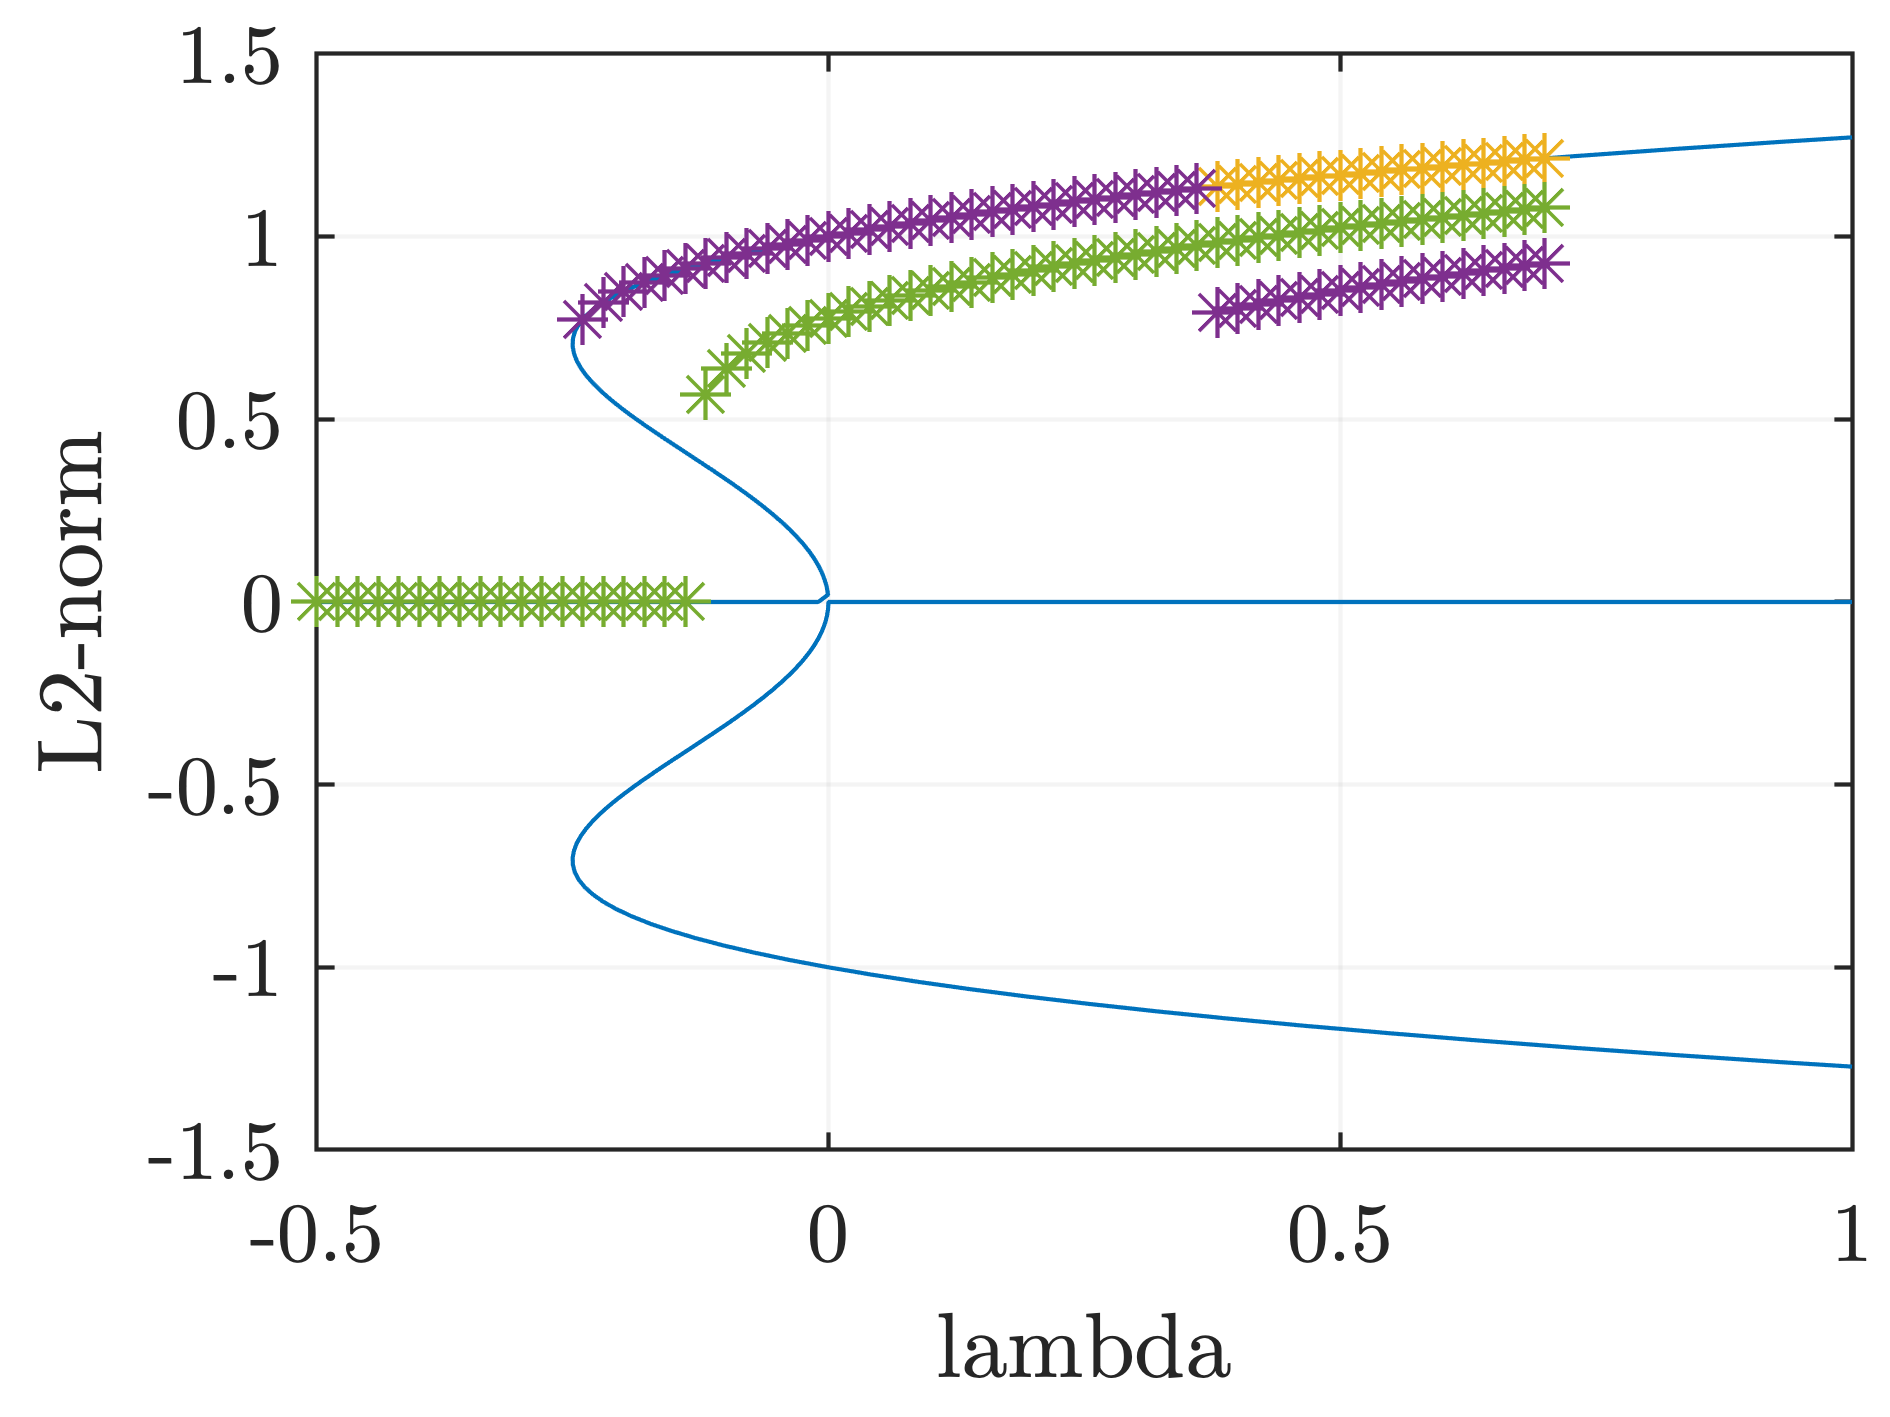
\includegraphics{bd_brute}
  \caption{Brute-force bifurcation diagram after \cref{question:bruteSigmoidal}.
  Asterisks denote brute-force continuation started from a homogeneous steady state
(yellow) a patterned ``bump" state (green) or a patterned sigmoidal state (purple)
for $\lambda = 0.7$, and continuing down to $\lambda =
-0.5$. The continuation jumps at several points, and some branches overlap (a yellow
and purple branch, for instance, lay underneath the green branch of trivial
homogeneous states $u(x) \equiv 0$). See solutions for a more thorough description.}
  \label{fig:bd_brute}
\end{figure}

\begin{question}(Preparing for numerical continuation)\label{question:prepare}
  You should now have a bifurcation diagram such as the one in \cref{fig:bd_brute}. 
  We will now prepare to perform a better form of numerical continuation: more
  reliable, and able to compute and classify stable as well as unstable states. Let us
  start by preparing initial guesses for $\lambda = 0.7$. Run 3 time simulations for
  $t \in [0,50]$ and $\lambda = 0.7$, so as to obtain approximations to: (i) a
  homogeneous steady state; (ii) a heterogeneous, stationary, bump state; (iii) a heterogeneous,
  stationary sigmoidal state. Save the solution profile $u( x, 50)$, as well as the parameters
  $p$ in a suitable \lstinline|.mat| file, which you will later reuse for
  continuation.
\end{question}

\begin{question}(Solving boundary-value problems) \label{question:fsolve}
  As seen in the lectures, any
  equilibrium of the PDE \cref{eq:AC} (irrespective of its stability), satisfies the
  boundary-value problem\footnote{Recall that in our notation, $\partial_{xx}$
  indicates, with a slight abuse of notation, both the partial derivative of a
  bivariate function, say $u(x,t)$, and an operator that maps a single-variable
function $u(x)$ to its second derivative. We are using the latter here.}
  \begin{equation}\label{eq:BVP}
    \begin{aligned}
      & \nu \partial_{xx}u + \lambda u + \alpha u^2 + \beta u^3 - \gamma u^5 = 0, \qquad x \in (-5,5), \\
      & \partial_x u(-5) = \partial_x u(5) = 0, 
    \end{aligned}
  \end{equation}
  or, in discrete form
  \begin{equation}\label{eq:BVPDiscrete}
    0 = \nu D_{xx}U + N(U,\lambda,\alpha,\beta,\gamma) =: F(U,p)
  \end{equation}

  For fixed $p \in \RSet^5$, one can approximate equilibria by solving the set of $n$
  nonlinear equations \cref{eq:BVPDiscrete}, using Newton's method, or one of its
  variants. This method of finding equilibria is alternative to time-stepping, and is
  at the heart of numerical continuation.

  Newton's method require evaluations of the function $U \mapsto F(U,p)$, and of the
  Jacobian matrix $U \mapsto D_UF(U,p)$, where $p \in
  \RSet^p$ is fixed.
%
  Recall that we have already coded the function $F$ in
  \lstinline|AllenCahn.m|. We can now amend this function, so as to return Jacobian
  evaluations when required. This new function can then be passed to Matlab's
  \lstinline|fsolve| function, which implements a variant of Newton's method. 

  \begin{enumerate}
    \item Compute with pen and paper the $n$-by-$n$ Jacobian matrix $D_U F(U,p)$.
      Express this matrix using $D_{xx}$ and a suitably-defined diagonal matrix
      containing the derivatives of $N$.

    \item Modify the function \lstinline|AllenCahn| so as to have the following
      interface 
      \lstinputlisting[lastline=1,numbers=none]{../Solutions/Code/AllenCahn.m}
      If \lstinline|nargout = 1|, the function returns only \lstinline|F|, as the previous
      version of the function \lstinline|AllenCahn|. If \lstinline|nargout = 2|, the function
      returns \lstinline|F| as well as the Jacobian matrix \lstinline|DFDU|. This
      means that all function calls below are now possible
\begin{lstlisting}[numbers=none]
>> F = AllenCahn(u,p,Dxx);
>> [F,DFDU] = AllenCahn(u,p,Dxx);
>> [~,DFDU] = AllenCahn(u,p,Dxx);
\end{lstlisting}
     This type of interface is also useful to pass functions to \lstinline|fsolve|.

    \item Use Matlab's in-built function \lstinline|fsolve| to solve the
      discretised boundary-value problem \cref{eq:BVPDiscrete}. You should aim to
      obtain a sigmoidal steady state for $\lambda = 0.7$, so you must set the
      parameter vector $p$ accordingly, and may select as initial guess the sigmoidal
      solution saved in \cref{question:prepare}, which is an approximation to the
      equilibrium. It is useful that the
      \lstinline|.mat| file stores the profile $u$ as well as the vector $p$, so you
      can pass $p$ directly the correct parameters to \lstinline|AllenCahn|.

      The function \lstinline|fsolve| interfaces with functions of the type 
      $U \mapsto F(U,p)$, and $U \mapsto D_UF(U,p)$, hence you should pass to it a
      function handle such as
\begin{lstlisting}[numbers=none]
  ACProblem = @(u) AllenCahn(u,p,Dxx);
\end{lstlisting}
      and set the option \lstinline|'Jacobian'| to \lstinline|'on'| to evaluate
      Jacobians. This will prompt \lstinline|fsolve| to call the function handle
      using either one of the two expressions below:
\begin{lstlisting}[numbers=none]
  F = ACProblem(u), [F,DFDU] = ACProblem(u);
\end{lstlisting}
      thereby implementing $U \mapsto F(U,p)$ and $U \mapsto D_UF(U,p)$. It is useful
      to examine other options of \lstinline|fsolve|, such as \lstinline|Display|,
      \lstinline|TolFun|, and \lstinline|MaxIter|, for instance.

    \item Plot the initial guess and solution to the BVP. Since the initial guess
      obtained by time simulation is close to an equilibrium, the functions should be very
      similar, and \lstinline|fsolve| should use only few iterations to converge.
  \end{enumerate}
  \end{question}

  \begin{question}[Perturb and find a new equlibrium]\label{question:perturbFsolve}
    In the previous question we found an equilibrium for $\lambda = 0.7$. We can use
    the same initial guess and attempt to find an equilibrium for another value of
    $\lambda$. Use the same initial guess and procedure of \cref{question:fsolve} to
    find an equilibrium for $\lambda = 0.4$. Since the initial guess is now less
    accurate (we are using as initial guess an equilibrium for $\lambda=0.7$ to solve
    the BVP for $\lambda = 0.4$), you should observe that convergence is achieved,
    but using more steps than before.
  \end{question}

  \section*{Intermezzo: recapitulation and remarks on numerical continuation} Let us
  pause for a moment to reflect on our results: we have now seen two strategies for
  computing curves of equilibria to the Allen--Cahn problem: (i) brute-force continuation
  is based on time stepping an initial condition long enough, until we obtain an
  equilibrium, and then using the final condition to time step a new problem, in
  which $\lambda$ is perturbed; (ii) the procedure outlined in
  \cref{question:fsolve,question:perturbFsolve} substitutes time stepping with
  solving a BVP.

  \lstinputlisting[basicstyle=\small\ttfamily,
                   float,
		   caption=Continuation demo for a scalar nonlinear problem,
		   label=lst:demo]{../Solutions/Code/continuationDemo.m}

  Numerical continuation adopts a strategy similar to (ii), that is, it computes
  equilibria using Newton's method. A full understanding of this tool is out of
  scope here: you are provided with a function implementing \textit{secant
  continuation}.

  The function \lstinline|SecantContinuation| takes the function $F$, and several
  other parameters associated to the continuation (see explanations in Listing
  \ref{lst:demo}), and produces a branch of steady states for the problem $\dot U =
  F(U,p)$, in the parameter $p(\text{\tt icp})$, using the Euclidean $2$-norm of $U$
  as solution measure. 

  In the example in Listing \ref{lst:demo} we show how to use \lstinline|SecantContinuation| to continue
  steady states of the scalar ODE $\dot U = \lambda U + \beta U^3 - U^5$ in the
  parameter $\lambda$.
  The function returns:
  \begin{itemize}
    \item A matrix \lstinline|bd| with \lstinline|nsteps|$+1$ rows and 3 columns:
      \lstinline|bd(1,:)| contains a label for points in the branch, from $0$ to
      \lstinline|nsteps|; \lstinline|bd(2,:)| contains values of the continuation
      parameter $p(\text{\tt icp})$; \lstinline|bd(3,:)| contains values of $\|U\|$.
      This matrix is useful to plot bifurcation diagrams.
    \item A matrix \lstinline|sol| with \lstinline|nsteps|$+1$ rows and $n$ columns:
      \lstinline|sol(i,:)| contains the steady state $U$ computed for $p(\text{\tt
      icp}) = \text{\tt bd(i,2)}$. This matrix is useful to fetch specific solutions
      on the bifurcation diagram, and post-process them.
  \end{itemize}

  \begin{question}[Continuation of sigmoidal equilibria] \label{question:sigmoidalBranch}
    We are now ready to re-compute the bifurcation diagram in \cref{fig:bd} with more
    generality. Compute a branch of sigmoidal
    steady states, and plot the resulting bifurcation diagram. It may be useful
    to start from one of the \lstinline|.mat| files saved in \cref{question:prepare}.
  \end{question} 

  \begin{question}[Continuation of bump equilibria]
    Compute a branch of bump steady states, and include it in the bifurcation diagram
    of \cref{question:sigmoidalBranch}.
  \end{question} 

  \begin{question}[Continuation of homogeneous states]\label{question:homBranch}
    Compute branches of homogeneous steady states, and include them in the bifurcation diagram
    of \cref{question:sigmoidalBranch}.
  \end{question} 

\vspace{3cm}
\begin{center}
  
\includegraphics[width = 0.3\textwidth]{spoiler}\\
  \textbf{The next page contains a spoiler. Do not turn the page before
  attempting \cref{question:homBranch}.}
\end{center}
\newpage

\begin{figure}
  \centering
  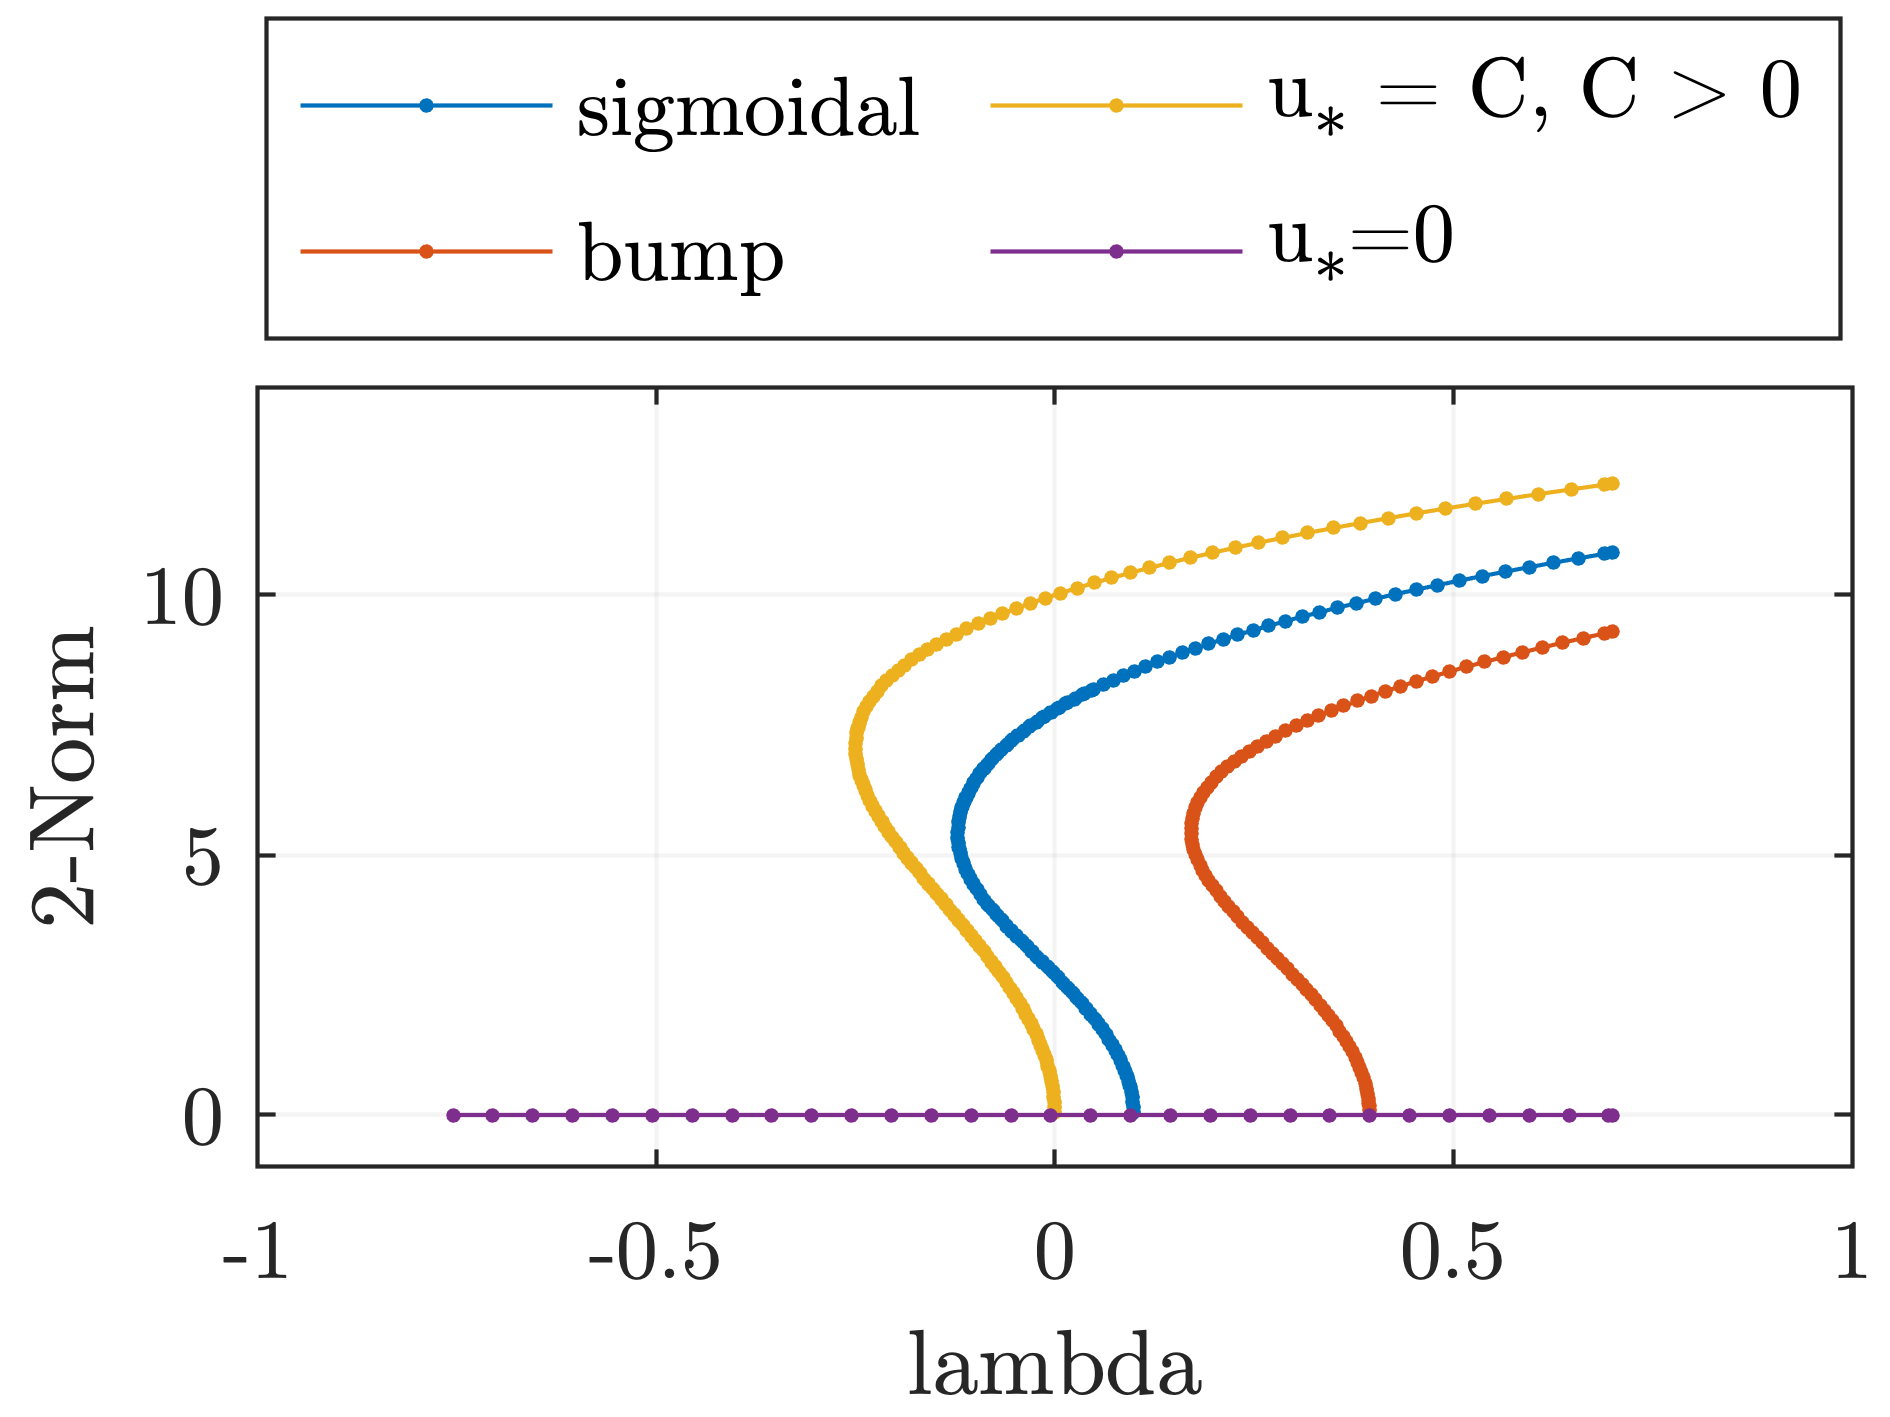
\includegraphics[width=0.8\textwidth]{bd}
  \caption{Selected solution branches of stead states of \cref{eq:AC}, obtained with
  numerical continuation.}
  \label{fig:bdCont}
\end{figure}

\begin{question}[Stability of $u_* \equiv 0$ (analytic)]\label{question:stabAna}
  You should have obtained a plot with
  various branches, as shown in \cref{fig:bdCont}, and we can now proceed to discuss
  linear stability. Using pen and paper, find an approximate linear evolution equation for small
  perturbations $v(x,t)$ of a steady state $u_*(x)$ of \cref{eq:AC}. Deduce that
  small perturbations around $u_*(x) \equiv 0$ evolve as
  \begin{equation}\label{eq:linear}
    \begin{aligned}
      & \partial_t v(x,t) = \partial_{xx}v(x,t) + \lambda v(x,t), && (x,t) \in (-5,5) \times \RSet_{> 0} \\
      & \partial_x v(\pm ,5) = 0,         && t \in \RSet_{\geq 0}.
    \end{aligned}
  \end{equation}
 
  Show that the branch of steady states $u_*(x) \equiv 0$ undergoes countably many
  bifurcations at $\lambda = \lambda_k$, $k \in \NSet$ (find an expression for
  $\lambda_k$), and with the corresponding critical modes  $\psi(x) = \psi_k(x)$
  (find an expression for $\psi_k(x)$).

  Verify that the 3 branches of nontrivial steady states in \cref{fig:bdCont}
  bifurcate from the branch of trivial steady states ($u_*(x) \equiv 0$) at $\lambda
  = \lambda_0, \lambda_1,\lambda_2$, respectively. You can do so by comparing the
  analytical values $\lambda_{0,1,2}$ to the plot.
\end{question}

\begin{question}[Stability of equilibria (numerical)]
  In this question we learn how to obtain information on the linear stability of a
  generic solution $u_*(x)$, by approximating eigenvalues and eigenfunctions of the
  linearised problem.

  Formally, if one casts the \cref{eq:AC} as
  \[
    \partial_t u = \calF(u,p) 
    \quad \textrm{on $(-5,5) \times \RSet_{>0}$},
    \qquad \partial_x u = 0 \quad \textrm{on $\{-5,5\} \times \RSet_{\geq 0}$},
  \]
  then the linear stability of an equilibrium $u_*$ attained for $p =
  p_*$ is studied via the linearised problem
  \[
    \partial_t v = \partial_u \calF(u_*,p_*) v
    \quad \textrm{on $(-5,5) \times \RSet_{>0}$},
    \qquad \partial_x v = 0 \quad \textrm{on $\{-5,5\} \times \RSet_{\geq 0}$},
  \]
  and, more specifically, by solving the eigenvalue problem
  \begin{equation}\label{eq:eigenProb}
    \partial_u \calF(u_*(x),p_*) \psi(x) = \mu \psi(x)
    \quad \textrm{for $x \in (-5,5)$},
    \qquad \partial_x \psi(\pm 5) = 0.
  \end{equation}

  In \cref{question:stabAna} we could solve the eigenvalue problem
  \cref{eq:eigenProb} analytically for the trivial solution $u_*(x) \equiv 0$, but
  this is the exception rather than the rule: in general one does not know $u_*(x)$
  in closed form, and hence can not solve \cref{eq:eigenProb}.

  The work done in the previous questions, however, puts us in a favourable position
  to study
  stability numerically: we have an approximation $U_* \in \RSet^n$ to
  $u_*(x)$, and we can solve the eigenvalue problem which discretises
  \cref{eq:eigenProb}, namely
  \begin{equation}\label{eigenProbNum}
    D_U F(U_*,p_*) \Psi = \mu \Psi
  \end{equation}
  where the $n$-by-$n$ Jacobian matrix $D_U F(U_*,p_*)$ encapsulates boundary
  conditions, and where $\Psi \in \CSet^n$ is an approximation to the eigenfunction
  $\psi(x)$.

  In fact,  we already have a routine that provides an approximation to the matrix
  $D_U F(U_*,\lambda_*)$ (see \cref{question:fsolve}): for a given solution
  \lstinline|u| and parameter set \lstinline|p|, this is obtained via the commands.
\begin{lstlisting}[numbers=none]
  [~,DFDU] = ACProblem(u,p,Dxx);
\end{lstlisting}
All we need to do to solve \cref{eigenProbNum} is calling Matlab's routine
\lstinline|eig| which computes eigenvalues and eigenfunctions of a matrix.

Use \lstinline|eig| to approximate eigenvalues and eigenfunctions for the trivial steady state
$u_*(x) \equiv 0$ for $\lambda = 0$. Use Matlab's command \lstinline|sort| to order
the eigenvalues according to the magnitude of their real part, in descending order.
\[
  \real \mu_1 \geq \cdots \geq \real \mu_{i-1} \geq \real \mu_{i} \geq \real
  \mu_{i+1} \geq \cdots \geq \real \mu_n
\]

Display the 5 most unstable eigenvalues $\{ \mu_i \}_{i=1}^5$ and plot the
corresponding eigenfunctions $\{\Psi_i\}_{i=1}^5$. Keeping in mind the results of
\cref{question:stabAna}, discuss with a colleague why these computations provide
numerical evidence of the following statement: 
\textit{the trivial stationary sate undergoes a bifurcation at $\lambda = \lambda_0 =
  0$, with critical eigenfunction $\psi_0(x) \equiv c_0$, for $c_0 \in \RSet$.}

\end{question}

\begin{question}\label{question:trivialInstabilities}
  Produce numerical evidence of the following statements:
 \begin{enumerate}
    \item the trivial stationary sate undergoes a bifurcation at $\lambda = \lambda_1 =
    (\pi/10)^2$; at this value of $\lambda$ the spectrum of the linearised operator has
    one unstable eigenvalue, and one eigenvalue at $0$; the equilibrium
    $u_*(x) \equiv 0$ for $\lambda = \lambda_1$ is unstable to perturbations
  $\psi_0(x) \equiv c_0$, and has critical eigenfunction $\psi_1(x) = c_1 \sin(
  \pi x/10)$, with $c_0,c_1 \in
  \RSet$.

  \item the trivial stationary sate undergoes a bifurcation at $\lambda = \lambda_2 =
      (\pi/5)^2$; at this value of $\lambda$ the spectrum of the linearised operator has
      two unstable eigenvalues, and one eigenvalue at $0$; the equilibrium
      $u_*(x) \equiv 0$ for $\lambda = \lambda_2$ is unstable to perturbations
    $\psi_0(x) \equiv c_0$, $\psi_1(x) = c_1 \sin( \pi x/10)$, and has critical
    eigenfunction $\psi_2(x) = c_2 \cos( \pi x/5)$ with $c_1,c_2,c_3 \in \RSet$.
  \end{enumerate}

\end{question}

\begin{question}
  With the tools built so far, you can explore in full the bifurcation diagram in
  \cref{fig:bdCont}. This question is more open ended than the others and leaves room for
  your initiative. It is important that you think of a way of addressing the
  question at large
  (numerical simulation, numerical bifurcation analysis, analysis, a combination
  thereof), and possibly formulate new questions by yourself. These are a selection of
  open questions you may consider (they all conceal subtleties and directions you
  are invited to explore): 
  \begin{itemize}
    \item Summarise what you have learnt about branches of steady states
      of the Allen--Cahn PDE.
    \item How many \textit{stable} stationary states does the Allen--Cahn equation suport for $\lambda =
      0.7$, and what is their spatial profile? What can we expect from a time
      simulation at $\lambda = 0.7$? Is your intuition backed-up by time simulations?
      What if $\lambda < 0.7$?
    \item Go back to \cref{fig:bd}. The bifurcation diagram with solution measure
      $S_1 = C$ displays solutions with $C<0$. What happened to them in
      \cref{fig:bdCont}? And do branches of of heterogeneous states have this
      behaviour too?
    \item Throughout our study we have set $\alpha = 0$. Can you formulate any conjecture,
      on any solution branch, for the case $\alpha \neq 0$?
    \item As in any PDE, boundary conditions have a strong effect on the dynamics:
      what would change if instead of homogeneous Neumann one imposes homogeneous
      Dirichlet boundary conditions?
  \end{itemize}

\end{question}

% \bibliographystyle{siamplain}
% \bibliography{references}
\end{document}
